%\documentclass[a4paper]{article}
\documentclass[a4paper,sfsidenotes]{tufte-book}
\usepackage{localstyle} % local style file

%\title{Using Authorization Logics To Model Security Decisions in Mobile Systems\\\vspace{2em}Thesis Proposal}
\title{Security Policies\\For Humans\\Thesis Proposal}
\author{Joseph~Hallett}
\date\today

\bibliographystyle{plainnat}
\begin{document}
\maketitle
\setcounter{tocdepth}{3}
\tableofcontents
\pagebreak

\section{Introduction}

\begin{marginfigure}
  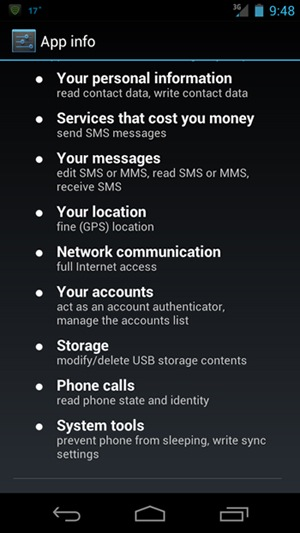
\includegraphics[width=\linewidth]{img/facebookperms.jpeg}
  \caption{Some of the permissions requested by the Facebook app.}
  \label{fig:fb}
\end{marginfigure}

When an app is installed on Android the user is prompted to accept the
privileges granted to the app.  The user makes the decision based on what they
know about the app and their own security policies.  Most users accept the
app without thinking about it.  They do this for a many reasons: because they don't
understand the risks, they don't understand the permissions, or they simply
don't care and will install the app whatever. Facebook is a good example of this
(Figure~\ref{fig:fb}) as the app requests a great many permissions but most
users trust it not to be malicious.  This is problematic because some apps are over
privileged\cite{Felt:2011kj} and some are malicious\cite{Zhou:2012cf}.  Other
apps are \ac{PUS} because though they are not malicious in
themselves they handle data in a way that is not in the user's interests.

More generally users and computers make decisions. Whether it is to update an
app or to connect to a website: the decisions are made based on the security
policies and trust relationships of the user and device.  These security
policies may include the use of tools or experts to decide whether something is
malicious.  For instance a user may trust a firewall program to enforce their
network policy; and they may trust a tool like \emph{Shorewall} to generate the
actual policy for them.  Alternately a user might wish to be able to install
apps but only trust apps \emph{Amazon} have vetted to be installed on their
device.  \emph{The aim of this project is to formalize these security policies
  so they can be studied and enforced automatically.}

Mobile operating systems are similar to existing systems but have a
different trust model and are used differently.  Software is
bought and downloaded from app stores, Apps run within sandboxes and collaborate and
collude to share data. The devices contain more personal data
than before: sensors tracking users' locations,  gyroscopes measuring how
users move, and microphones listening to users calls.  The \ac{BYOD} trend
encourages users to take the devices they have at home into work.
This creates a tension between how the corporate IT department may require
employees to use their devices and the user's policies on how they want to use
their devices.  These features add a novel challenge to modelling these devices
and the stores and users surrounding them.  

Formalizing policies allows comparisons to be made between different systems
and the user's policies.  When we compare the two biggest mobile OSs,
iOS~and~Android, the comparisons is informal: iOS is more closed, more of
a \emph{walled garden}, Android is more permissive.  With a formal language to
describe system policy we can make a precise comparison. 

There has been much research on static analysis tools.  These tools infer
complex security properties about the code.  What is missing is the link between
the assurances these tools can give and the policies users are trying to
enforce.  By using an \emph{authorization logic} as the glue layer we can
enforce the policy by building on the work on access control in distributed
systems.  Static analysis tools can be trusted to give statements about code, as
can other analysts and principals, that can be combined to implement a security
policy.

This thesis aims to show how authorization logics can be used to make
security decisions in mobile devices.  Security decisions are made
manually by smart phone users and it is our belief that by automating these
choices users can avoid having to make security decisions and their overall
security be improved.  To do this we plan to look at the following areas: 

\begin{itemize}
  \item \emph{To model the decisions and trust relationships inherent in Android
      and other mobile operating systems.}  We will write a
    security policy that describes the current state in these systems and serve
    as a base to compare other systems against. 

  \item \emph{To instantiate a logic of authorization that allows us to model
      the trust relationships between the components of an operating system and
      the users.}  This will include analysis tools as principals and allow
    making decisions based on signed statements from them.  The logic must be
    able to model what happens when apps can collude.  The logic may be based
    off of earlier work on the \emph{SecPAL~language}\cite{Becker:2006vh} that
    was used for distributed access control decisions.

  \item \emph{To implement an app store that serves users only the apps that
      meet their security policies.}  This will include a user-study where we
    evaluate how well users comprehend their policies and the decisions made for
    them. This may lead into generating proof-carrying code certificates for
    apps that allow a device to check that their policy was met without having
    to do the full inference themselves.

  \item \emph{To study how users understand their security policies and the
      ways these policies are enforced.}  One of the advantages of SecPAL is
    that it is more readable compared to other authorization logics and access
    control languages.  Whilst end-users might not want to write their own
    policies they should be able to comprehend what a policy means, and they
    should be able to understand why their policy allows some decisions and not
    others.

  \item \emph{To explore how security policies change with time and when apps
      can collude.}  A user's security policy need not be static.  People change
    jobs and may bring old devices to new environments requiring new security
    policies.  Apps can collude: two apps might meet a security policy when
    considered on their own but together they might act to share data
    inappropriately.  Over time an app might want greater access and increased
    permissions to support new functionality.  It is not obvious how to write
    and check security policies written in SecPAL for these scenarios and how
    to enforce the policy at runtime.

\end{itemize}

\subsection{A Logic of Authorization For Mobile Devices}

Logics of authorization decide whether an entity may do something. This might be
carrying out an action, accessing data, or describing what another entity can
do. When we apply these logics to files and information we create an access
control system; when we apply the logics to designing systems we create a
security specification language.  A review of the history and applications of
the logics is given later in this proposal (page~\pageref{sec:pollang}); but in
summary they have shown themselves to be increasingly useful for modelling the
complex security and trust policies in modern systems.

Mobile devices are different to traditional computers. They have more
information about their users. They don't offer the user the traditional file
system interfaces. Everything is sandboxed and closed software markets (app
stores) distribute software.  The app stores typically allow developers to sell
their apps but are selective about what they will sell.  Apps are vetted for
quality and security\footnote{We believe: very few stores document their
  policies.  The \emph{Firefox Marketplace} is a notable exception as they
  publish their review criteria online.
  \url{https://developer.mozilla.org/en-US/Marketplace/Submission/Marketplace_review_criteria}}.
  Static and dynamic analysis tools are used as well as traditional inspection.
  The policies the app stores apply to their apps form an authorization decision
  (\emph{the analysis team says app can be sold}) and there is a delegation of
  trust to the analysts and their tools. It is not clear how these policies and
  trust relations filter through to the end users.

These differences amount to a different model of trust
than the traditional machines, and a new set of authorization problems that it
is not obvious how to express in other authorization logics. 

To solve this we have taken an existing authorization logic,
SecPAL\cite{Becker:2006vh}, and extended it with a series of predicates that can
describe how security policies are met inside a mobile ecosystem.  Future work
will include describing the current security policies for Android and other
mobile OSs as well as the app acceptance policy for some app stores.  This will allow comparisons to be
made between them, and (with a database of apps) comparing what kinds of apps
different markets allow.

\subsection{Compositional Policies Over Time}

Consider a user who has a smart phone and is buying apps.  The
user must decide if they want to install an app: to do this they apply a series
of judgements called their \emph{security policy}.  

The user has their own security policy. They also have other security policies
they implicitly follow.  When they download apps from an app store they also
gain the security policy of the store and what it will sell.  If the phone runs
in a corporate environment then they may also be subject to the company's
corporate policy.  The operating system itself may have certain restrictions on
what it will allow.  The APK app format used on Android can also be installed on
Blackberry and Sailfish operating systems.  Each system may add
additional restrictions that may make some apps not installable.  An example of
how a compositional policy might be written is shown in
Figure~\ref{example:composition}.

\begin{marginfigure}\label{example:composition}
  \begin{lstlisting}[language=SecPAL]
Phone says app is-installable
  if app meets UserSecurityPolicy,
     app meets AppStorePolicy,
     app meets ITDeptPolicy,
     app meets OSPolicy.

Phone says User can-say inf
  app meets UserSecurityPolicy.

Phone says PlayStore can-say 0
  app meets AppStorePolicy.

Phone says ITAdmin can-say inf
  app meets ITDeptPolicy.
  \end{lstlisting}
  \caption{A compositional security policy where an installation policy for a
    phone is dependent on other security policies.}
\end{marginfigure}
     
The phone might use this policy for a while, but then the user changes jobs.
Now they have to meet a new \code{ITDeptPolicy} set by a different administrator.
Should any installed apps be uninstalled if they don't meet the new policy?  If
we already have a certificate showing the apps passed the old policy can we
reuse it to create a new certificate that shows the app meets any additional
restrictions?

Whilst other authorization logics have looked at making one-time decisions about
whether to allow a computer to make a decision; there has been less work on
modelling these policies over time and seeing how a changing security policy
affects a changing device.  This could add novelty.

Alternatively say there is an app which the developer is continually improving
and adding new features.  When the app is installed it may meet the security
policy but with increasing features requiring access to more permissions and
introducing more complexity or a change of advert library the app no longer
meets the security policy.

Should the app be removed?  If the app is used every day by then the user may
not be pleased that the phone has decided to break their favorite
app; though anecdotal evidence would suggest users tend to blame apps
  for failing rather than the frameworks they apps rely on; regardless of who is
  really to blame. Equally just stopping updates for the app increases app
version fragmentation and reduces security by rejecting bug fixes.  Allowing the
update isn't correct either as it allows a means to break the security policy.

Whilst there have been several papers looking at (and proposing methods to stop)
excessive permissions in applications\cite{Felt:2011kj}\cite{Vidas:2011wr} there
has not been a thorough review of how permissions change for apps over time
and between versions of the same app. 

% TODO ADD BIT EXPLAINING HOW TO DO THIS


\subsection{Personally Curated App Stores}

Apps are normally distributed on mobile devices through an app
store.  On iOS users have the \emph{App Store}: a curated market place run by
Apple (though other, albeit clunkier, distribution mechanisms do exist for even
non-jail broken phones) that is perceived as being picky about the apps it sells.

Android users have a far greater choice of marketplace.  The \emph{Play Store}
is the app store distributed by Google. It is less moderated than Apple's store.
Amazon have their own app store that serves as a more curated version of
Google's offering. It is the default on their Kindle tablets.  Other app stores
target specific regions: such as \emph{gFan} in China, and the \emph{SK~T-Store}
in Korea.  Some, such as \emph{Yandex.Store, AppsLib and SlideMe}, are
pre-installed by OEMS who can't or don't want to meet Google's requirements for
the PlayStore.  The \emph{F-Droid} store only delivers open source apps. Others
exist to distribute pirated apps. 

On average eight percent\cite{AQUILINO:2013wr} of the apps in each of these
alternative market places is malware. The Play Store contains very little
malware however (0.1\% of total apps), whilst a third of the app in the
Android159 store were found to be malicious.

Every app store has a different security policy.  They enforce these
policies when they pick which apps to sell to their users.  By using an
authorization logic to decide whether apps will meet a security policy we have
the ability to create a new kind of app store where offerings are tailored to
the user's security policy.  By creating app stores tailored to a security
policy we also give ourselves a way to empirically measure how restrictive a
security policy is: we can measure the number of apps offered inside the stores.

To enhance trust in the store digital evidence could be offered
with the apps This would give devices a practical means to check the app is
supported by their security policy without having to re-run all the static
analysis checks
themselves. This should also save device battery life.  

Proof-carrying authentication\cite{Appel:1999dq} and authorization logics such
as BLF\cite{Whitehead:2004bu} have already introduced ideas from proof-carrying
code into authorization logics. The focus of their work has been on
access control where a user is providing a proof that they have the credentials
to access a resource.   In the scenario we propose the role of the user is
reversed: the store offers many proofs to the user to increase their trust in
its wares; rather than the user offering one specific proof to prove they have
the right to complete a certain action.


\subsection{Project Context (App Guarden)}

\begin{figure}\label{fig:ag}
  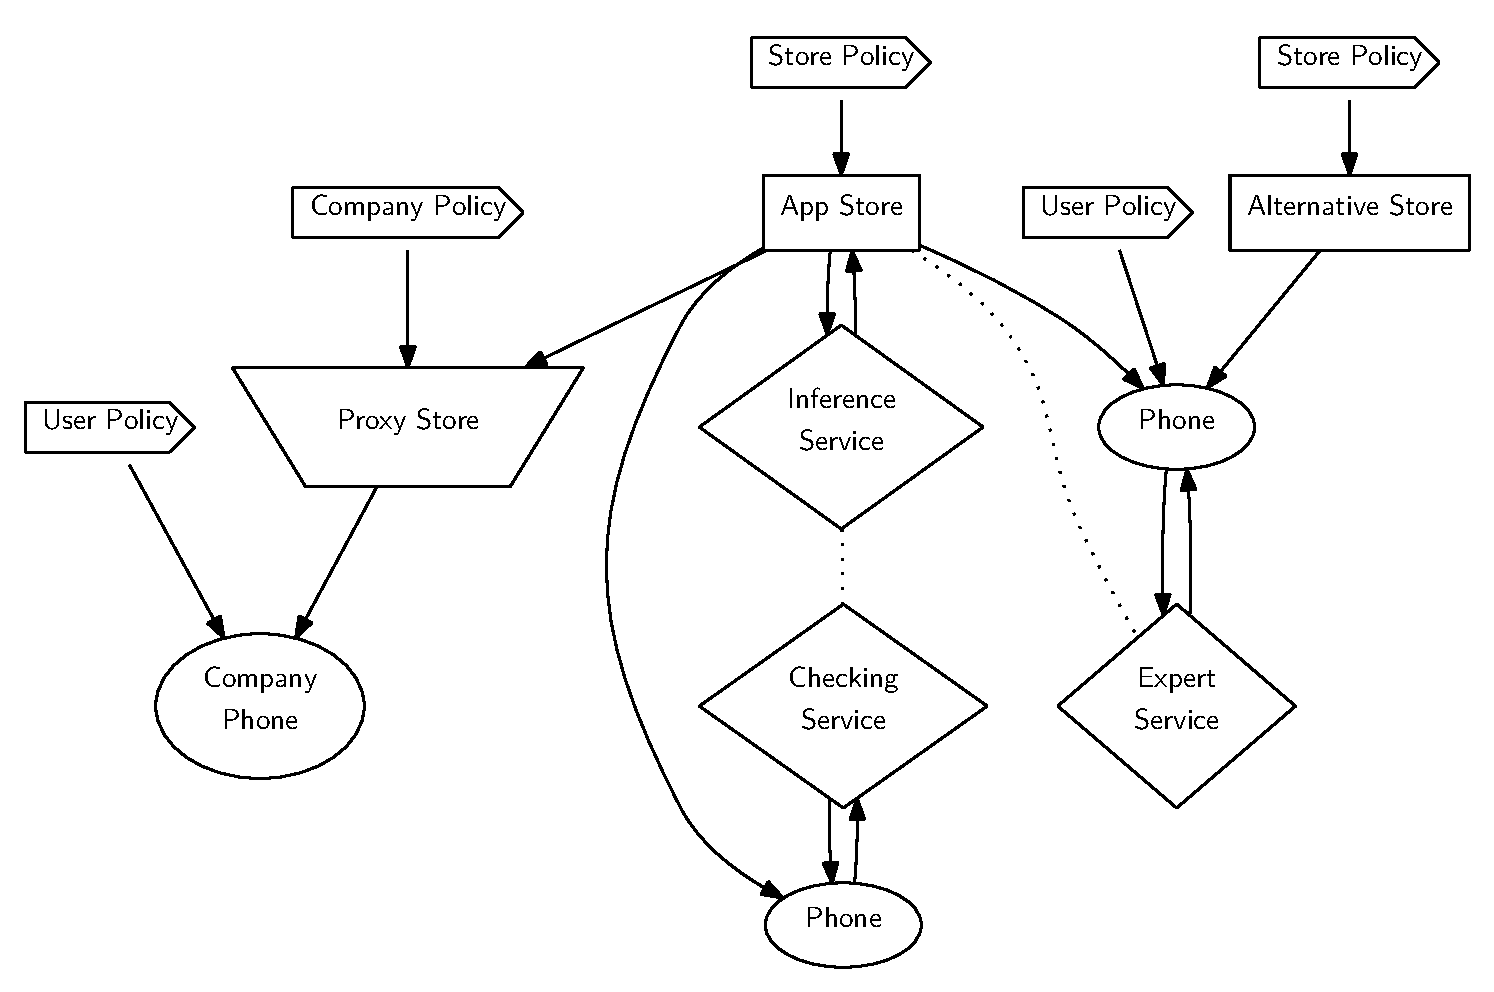
\includegraphics[width=\linewidth]{img/appguarden.eps}
  \caption{Overview of the different entities in App Guarden.  Each of the ovals
  represents a different device inside the system; each rectangle or trapezium
  represents  different supplier of apps, and each diamond is an authority that
  makes statements about apps and other software decisions.  Arrow boxes show
policies.  Arrows represent transfers of information or apps, and dotted line
indicate that the two entities are connected in some other way.}
\end{figure}

This thesis will form part of the \emph{App
Guarden}\footnote{\url{http://groups.inf.ed.ac.uk/security/appguarden/Overview.html}}
project.  The App Guarden project aims to improve the quality of mobile security
by developing new tools to analyze apps and the app stores that sell them.

This work contributes to this by developing the security policies that describe
what the user wants and showing how they can be enforced using the tools that
can check security policies within the code.  The end result might be a system
as shown in Figure~\ref{fig:ag} where devices are interacting with stores and
security services such as static analysis tools or proof checkers. 

\begin{marginfigure}
  \label{fig:proxy}
  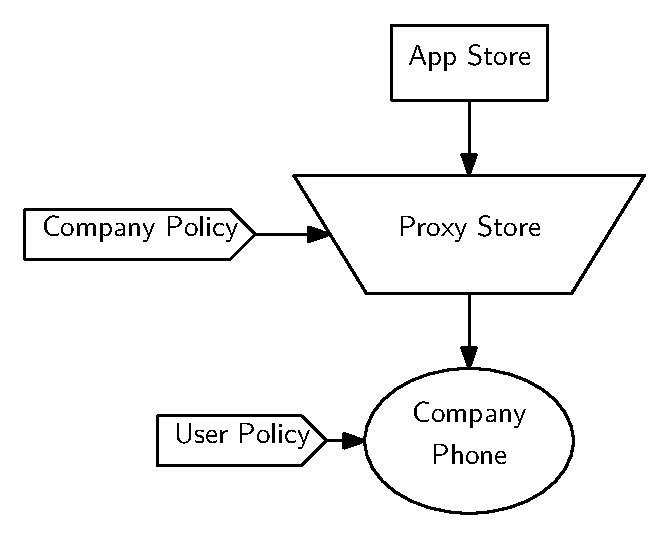
\includegraphics[width=\linewidth]{img/proxystore.eps}
  \caption{Security policies and the proxying store}
\end{marginfigure}

\begin{marginfigure}
  \label{fig:de}
  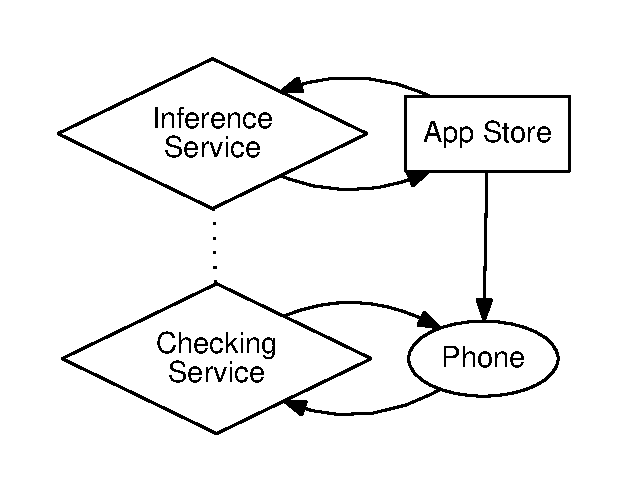
\includegraphics[width=\linewidth]{img/digitalevidence.eps}
  \caption{Checking services and an app store.}
\end{marginfigure}

\begin{marginfigure}
  \label{fig:mcafee}
  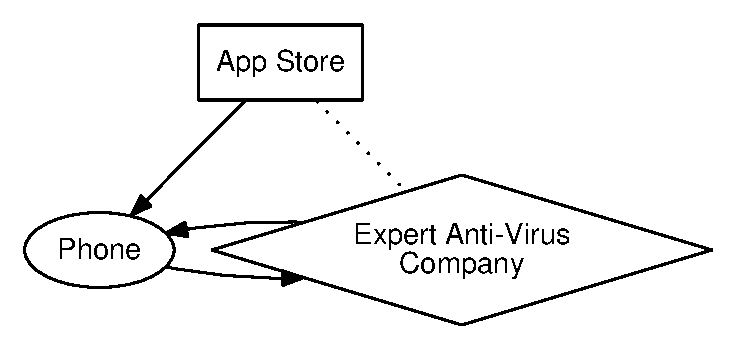
\includegraphics[width=\linewidth]{img/mcafee.eps}
  \caption{Use of an expert checker.}
\end{marginfigure}

\begin{marginfigure}
  \label{fig:altstore}
  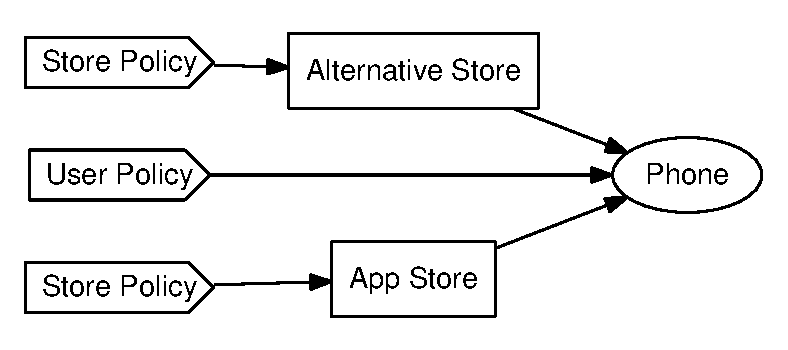
\includegraphics[width=\linewidth]{img/altstore.eps}
  \caption{A device using multiple stores with different policies.}
\end{marginfigure}

Between each of the nodes different policies could be enforced.  Consider an
\emph{app store} and \emph{proxy store}.  There is a master app store that sells
many apps.  A company provides its employees each with a phone that they can
install apps on but they have their own security and usage policy set by their
IT department.  Employees shouldn't install anything that breaks the policy. On
all the devices the IT department provide they install a special proxy app
store.  The proxy app store takes apps from the main store but discards any apps
which might break the policy it is supplied with.  Users may download apps from
the company store, but they might exercise their own judgement and only download
apps that meet their own policies.  At each stage (as shown in
Figure~\ref{fig:proxy}) judgements are being made about what is acceptable from
an app store, and the policies are refined.

Another example might be an app store that supplies apps with \emph{digital
evidence}.  When the app store sells an app it wants to reassure its users that
it real guarantees that the app it is selling meets the security guarantees it
claims.  Being able to infer these properties is complex and takes both time and
battery power; this is difficult as many phones are battery constrained.  To
avoid this the app store uses an inference service to produce digital evidence
to be supplied with the app that shows (with the aid of a checking service that
could be running on the device) that an app meets the policy (as shown in
Figure~\ref{fig:de}). Other projects in the App Guarden project are 
developing these tools.

An alternative form of this could be where a store delegates to an expert third
party to make statements about the apps it sells.  One might imagine a scenario
where an app store might claim \emph{``We don't sell viruses in our store, but
don't take our word for it: here's a well known anti-virus company that will
verify our claim''} (as shown in Figure~\ref{fig:mcafee}).

If a user is using multiple stores (for example a jail broken iPhone user might
buy apps from both the App Store and the Cydia Store) then the policies the user
might be applying become complex (as described in Figure~\ref{fig:altstore}).
This leads to interesting questions around how policies should be composed and
the equivalence of security policies when they are; as well as questions about
the overall device policy in a system.

The work for this thesis will not concern itself with the development of tools
to check the apps perform as they should; rather it will focus on modeling the
trust relationships between these tools and the other entities in a mobile
environment.  This allows this part of the work to focus on the relationships
and device policies rather than the intricacies of code analysis.


\section{Review of Android Security}

Android is a Linux OS for mobile phones and
consumer electronics. It has a large software
market distributes apps. Apps on the Dalvik virtual machine.  Dalvik is a
modified JVM architecture: it uses registers rather than stacks to save memory;
and drops some type information (again for space).
Apps use a sandbox provided by the OS that is based on
Linux's permissions model\cite{Drake:2014uq}.

\subsection{Permissions and Apps}

\begin{marginfigure}\label{img:brightestflashlight}
  \centering
  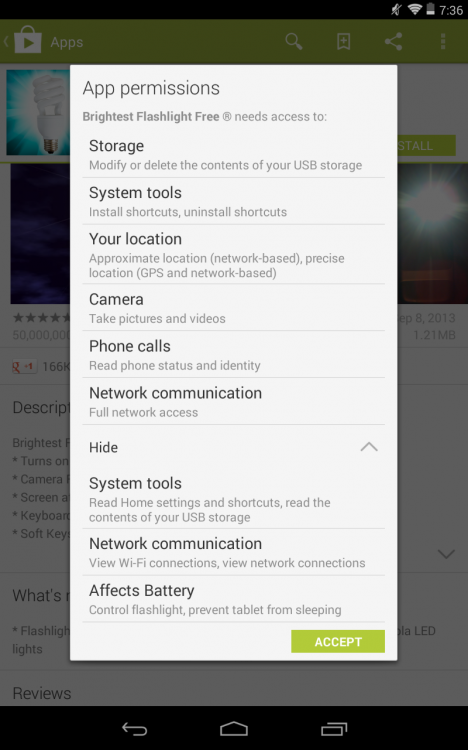
\includegraphics[width=0.8\textwidth]{img/brightestflashlight.png}
  \caption{The \emph{Brightest Flashlight Free} app prompting for its permissions
    at install time. This app is over privileged as a flashlight app should have
    no need for GPS or phone data, or network access.}
\end{marginfigure}

Android has API permissions that apps must request at install time. API
permissions control access to things such as the internet, access to storage, or
to see the state of the phone. The permissions are shown at install time. If the
user disagrees with the permissions it cannot be installed. Users do not look at
these permissions; they accept them whatever is asked for\cite{Felt:2012hm}.
This has led to malware and \ac{PUS} that asks for too many permissions. This
lets bad apps send premium text messages (a common monetization
strategy\cite{Chien:2011vw}) or stealing private information.

Tools can detect when an app is over privileged (like the app in
Figure~\ref{img:brightestflashlight}). The \emph{Stowaway}
tool\cite{Felt:2011kj} mapped Android permissions onto the API calls. This
allowed them to detect when apps were over privileged by looking for those with
the permissions but not the associated API calls. The \emph{PScout}
tool\cite{Au:2012ju} improved upon Stowaway.  It did this by increasing the
accuracy of the permissions map. They built their map from the Android source
code; whereas Stowaway used fuzzing.

API permissions are quite broad. 
The \emph{internet} permission allows an app to send or receive anything on the
internet. Several people have proposed a \emph{finer grained permissions model}.
For example: the internet permission could limit which addresses an app could
talk to; similar to dependant typing.

The \emph{RefineDroid, Dr.~Android \& Mr.~Hyde} tools\cite{Jeon:2012ki} discover
which permissions can be made finer, rewrite apps to use these permissions and
then enforce them at runtime; they do this on a stock Android without needing
rooting. The \emph{AppFence} tool\cite{Hornyack:2011wq} doesn't modify apps.
Users can write policies for what data an app can receive. If an app breaks this
then the it is stopped or fake data supplied instead.  This requires changes to
Android however. The \emph{AppGuard} tool\cite{Backes:2013ec} rewrites apps to
use a security monitor. AppGuard does not require rooting.

\subsection{Intents and Collusion}

Android uses a novel IPC mechanism called \emph{Binder}. Apps use \emph{intents}
to share data and handle events. If an app wishes to handle an
\code{SMS_RECEIVED} action it declares itself a \emph{broadcast receiver} for
the action; the app will be started when the event occurs.  If an app wants to
open a web page it can send an \code{ACTION_VIEW} intent. The user's browser
will take open the URL.\@ Apps can create their own intents. They can restrict
usage of them to those signed with the same key.

Binder allows apps to collude to increase their privilege levels.  Consider two
apps communicating: one which can use the network and another which cannot.  The
unprivileged app asks the privileged app to send data on its behalf. The
privileged app forwards the network responses back to it. The unprivileged app
now has the network permission without declaring it to the user.  If a
privileged app does not secure its intents then they may break the protections
offered by permissions. The \emph{Kies} app by Samsung could be exploited like
this to install other apps\cite{moulu:8btkPowj}.

Tools have been made to find privilege escalation attacks.
\emph{Quire}\cite{Bugiel:2012ui} added origin tracing to intents.
\emph{ScanDroid}\cite{Fuchs:2009vi} statically analyzed apps to find flows
across components. It describes constraints that should be satisfied to stop
leaks. \emph{Kirin}\cite{Enck:2009ko} certifies apps at install time based on
the data-flows introduced by the requested permissions.

\emph{TaintDroid}\cite{Enck:2010uw} and \emph{FlowDroid}\cite{Fritz:2013vi}
have been influential.
Taint analysis is used to track
data passed between apps. They detect when sensitive data is being leaked to an
app. Others have shown
that the approach is not perfect\cite{Sarwar:2013ta}: it can be defeated by
malicious apps.

% TODO: INCLUDE SECTION ON ANDROID ROMS AND MALWARE

\section{Review of Policy Languages}\label{sec:pollang}

\subsection{Logics of Authorization}

When actions are performed, such as reading a file or installing an app,
conditions must be met for it to go ahead. These form the
\emph{authorization~policy} for the decision. When these policies describe what
is needed to keep a secure system it is called the \emph{security~policy}.  The
policies can contain \emph{trust} statements. Principals may be trusted to make
statements about others and what is allowed.

Early authorization logics, like \emph{PolicyMaker}\cite{Blaze:dj}, grew out of
the logics of authentication proposed by
\citeauthor*{Wobber:1994dh}\cite{Lampson:1992jg}\cite{Wobber:1994dh}.
PolicyMaker allowed other principles (identified through asymmetric keys) to be
trusted for actions or to declare further relationships. The language was
minimal. It did not specify how the policies should be checked: they suggested
regular expressions, or  a special version of AWK. Any language could have been
used, however.  The author suggested it might work well as a model for the
public-key infrastructure. Later work introduced
\emph{KeyNote}\cite{Blaze:1999fa} which was a simplified version of PolicyMaker
for public-key infrastructure.

Later languages like \emph{RT}\cite{Li:2002if} built on this. RT allowed
principals to be given roles; similar to a \ac{RBAC} system. Decisions
were made based on which roles were held. RT could express statements
that were not possible in PolicyMaker: \begin{quote} ``Anyone who is a
  preferred customer and a student can get a discount.'' \end{quote} Several
versions of RT were described: the simplest being \emph{RT$_0$}\cite{Li:2003tj}
and with \emph{RT$_1$} and \emph{RT$_2$} adding support for parameterized-roles
and logical-objects respectively. Extensions added support for constraints.

The RT family is known to be tractable as it can be translated into
\emph{Datalog} (specifically \emph{Datalog with constraints}; also called
\emph{Datalog$^C$\cite{Li:2003ix}}).  Datalog is known to be tractable. This is
unlike PolicyMaker which was not tractable in general. Datalog is a query
language similar to \emph{Prolog}. Datalog does not support nested sub-queries
or functions. It has a safety condition that all variables in the head must
occur in the body. These constraints make Datalog a subset of first-order logic.
Datalog queries can be done in polynomial time.

\emph{Cassandra}\cite{Becker:2004fi} was influenced by the RT family of
languages and Datalog$^C$.  Cassandra was a trust management system used to
model large systems.  In his doctoral thesis Becker showed how the NHS Spine
could be formally modelled in the Cassandra language.  The Spine is a complex
and informally defined system: it describes the jobs and responsibilities of NHS
employees.

In Cassandra principals activate and deactivate roles. Actions can only be completed if the
principal holds the required roles. Delegation is allowed through an
appointment mechanism. One principal can activate roles on other
principals. Cassandra is tractable as it can be translated
to Datalog$^C$.

\begin{marginfigure}\label{code:cassandra}
  \begin{align*}
    &\textsf{canActivate}(mgr, \texttt{AppointEmployee}(emp)) \\
    &\;\;\gets \textsf{hasActivated}(mgr, \texttt{Manager}()) \\
    &\textsf{canActivate}(emp, \texttt{Employee}(app)) \\
    &\;\;\gets \textsf{hasActivated}(app, \texttt{AppointEmpolyee}(emp))
  \end{align*}
  \caption{Role delegation in the \emph{Cassandra} policy language. A manager is
  allowed to activate the employee role for an arbitrary entity by appointing
  them.}
\end{marginfigure}

The \emph{Binder} language\cite{DeTreville:2002ff} was designed for
authorization decisions\cite{Abadi:2003kt}.  It is implemented as an extension
of Datalog.  Properties are predicates. Predicates refer to entities.  A
\emph{says} modality allows statements to be imported.  If a predicate can be
inferred from the knowledge base it is authorized.  Binder does not add any
predicates for handling state.  The version of Datalog used does not allow for
constraints.  This limits Binder's usability.


\emph{{SecPAL}}\cite{Becker:2006vh} is an authorization logic for decentralized
systems. Early experiments indicate that it is good  for modeling the
distributed nature of software installation, app stores and mobile devices. We
will describe it in more detail than other languages.

\begin{marginfigure}\label{code:binder}
  \begin{lstlisting}[language=Prolog,morekeywords={*,says,:-}]
can(X, read, file) :- 
  employee(X, company).
employee(X, company) :- 
  hr says empolyee(X, company).
hr says employee(john, company).
  \end{lstlisting}
  \caption{Statements in \emph{Binder} to say that in the current context only
    employees can read a file, and that an employee they must have a statement
    from HR to prove they are an employee.}
\end{marginfigure}

Syntactically {SecPAL} is similar to Binder. It has a richer syntax
that allows for constraints; and it can make decisions based on state (such as the
time). {SecPAL} was designed to be readable: it has a verbose, English like,
syntax than other authorization logics.

Like Binder it has a \emph{says} statement. Unlike Binder it requires that all
statements are said by a principal explicitly. {SecPAL} allows arbitrary
predicates to be created. It adds two additional special modalities to the
logic. The \emph{can-say} statement allows for explicit delegation and has two
varieties.  The \emph{can-say$_\infty$} phrase allows for nested delegation,
whereas the \emph{can-say$_0$} statement does not. {SecPAL} adds a
\emph{can-act-as} phrase that allows for aliasing entities; its use is limited
however.

Extensions of {SecPAL}\cite{Becker:2009vt} add support for guarded
universal quantification. They also remove the \emph{can-act-as} statement. Other
languages such as \emph{DKAL}\cite{Gurevich:2008fz} built on and eventually split
from {SecPAL}. DKAL was designed to express distributed knowledge between
principals by adding to the trust delegation mechanisms already in {SecPAL}.
They also showed how any {SecPAL} statement could be translated into {DKAL}.
The \emph{{SecPAL}4P} language\cite{Becker:2009ula} was an instantiation of (the
extended version of) {SecPAL} designed to specify how users' wished their
\ac{PII} to be handled.

The inference rules for SecPAL are shown in Figure~\ref{secpal:rules}. Queries
are evaluated against a set of known statements (the \ac{AC}) and an initially
infinite delegation level ($D$). If the rules show that the query is valid then
SecPAL says the statement is okay else it is rejected.

\begin{figure}\label{secpal:rules}
  \centering
  \begin{eqnarray*}
    \infer[\textsf{\scriptsize cond}]{%
      AC, D \models A\textsf{~says~}fact\theta
    }{%
      \begin{array}[c]{c}
        \left(A\textsf{~says~}\textit{fact}\textsf{~if~}\textit{fact}_1, \ldots, \textit{fact}_k, c\right) \in AC \\
        AC,D\models A\textsf{~says~}\textit{fact}_i\theta \; \forall i \in \{1\cdots k\}
      \end{array}
      & \models{c\theta}
      & \textsf{vars}(\textit{fact}\theta) = \emptyset)
    }\\
    \infer[\textsf{\scriptsize can say}]{%
      AC, \infty \models A\textsf{~says~}\textit{fact}
    }{%
      AC, \infty \models A\textsf{~says~}B\textsf{~can~say}_D \textit{fact}
      & AC, D \models B\textsf{~says~}\textit{fact}
    } \\
    \infer[\textsf{\scriptsize can act as}]{%
      AC, D \models A\textsf{~says~}B~\textit{verbphrase}
    }{%
      AC, D \models A\textsf{~says~}B\textsf{~can~act~as~}C
      & AC, D \models A\textsf{~says~}C~\textit{verbphrase}
    }
  \end{eqnarray*}
  \caption{The inference rules used to evaluate {SecPAL}. All {SecPAL} rules are
  evaluated in the context of a set of other assertions $AC$ as well as an
  allowed level of delegation $D$ which may be $0$ or $\infty$.}
\end{figure}

%\subsection{Access Control Systems}
% TODO
%{\Huge TODO}

\section{Review of Datalog}

Datalog is a database language. It was created from a simplification of general logic
programming.  The language is based on first order logic; it is both sound and
complete.  Datalog is used as the basis for several of the authorization
logics including SecPAL. We will review several evaluation strategies used
for querying Datalog knowledge bases.

\begin{marginfigure}
  \label{datalog:example}
  \begin{lstlisting}[language=Prolog]
person(alice).  
person(bob).
person(claire). 
person(david).
mother(alice, claire).
father(alice, david).
mother(bob, claire).
father(bob, david).
sibling(X,Y) :- person(X),   person(Y),
                person(M),   person(F),
                mother(X,M), mother(Y,M), 
                father(X,F), father(Y,F).
  \end{lstlisting}
  \caption{A simple Datalog program and describing a family, and a relation
  describing what it means to be a sibling.}
\end{marginfigure}

Datalog programs are presented as series of Horn~clauses in the syntactically
same way as the Prolog language (see Figure~\ref{datalog:example}).  There are
additional restrictions, however, that all variables in the head of a clause
must be present in the body; and that no parameter can be a nested predicate.

Datalog programs are split into two sets.
The \ac{EDB} has all ground (containing no free variables) facts.
The \ac{IDB} has rules for deriving more facts.

\subsection{Evaluation Strategies}

The \emph{bottom-up} or \emph{Gauss-Seidel} method is a simple evaluation
strategy\cite{Ceri:1989ff}.  Given a Datalog program try every constant with
every rule from the \ac{IDB}.  When a rule is found to be true add it to the set
of facts.  Repeat until a fixed point (or the required fact) is known.  If a
queried fact is still unknown when it stops then it is false; as Datalog assumes
the \ac{CWA}.  The strategy is complete and will always
terminate. Querying the database is fast once all facts have been inferred 
and large joins are quick.

This strategy ends up computing all known facts. It is less useful when only a
subset are interesting.  The \emph{magic sets}\cite{Bancilhon:1985cz} rewriting
rule avoids this problem.  Interesting constants are marked as \emph{magic}. The
knowledge base is a graph: nodes related to a magic one are also magic.  Rules
in the \ac{IDB} are rewritten to check constants used in the inference are also
be magic.  This cuts down on irrelevant results: anything that isn't
interesting will not be in the magic set.

The \ac{SLD} resolution algorithm works top down. It starts with a goal and then
constructs a proof tree. Transitions are applications of rules from the
\ac{IDB}. Nodes are either facts (the leaves) or further branches.  If there is
a subtree from the query node to true facts then it is true.  The Prolog
language (which Datalog is a more constrained form of) uses this strategy.  Its
use of memory efficient as it searches the tree in a depth-first manner.
Breadth-first and other tree traversal searches are also possible as are
parallel strategies.  The \emph{top-down} strategy is less commonly used with
Datalog programs. Tabling is often used with this strategy to speed queries by
memoizing previously inferred facts.

The \ac{SLD} resolution may
not terminate if there are a set of rules that set up an infinite loop (for
instance the rule \code{a(X) :- a(X).}).
Because Prolog has an infinite number of constants
(integers for example) it is possible to construct queries which return an infinite
number of answers.

\subsection{Datalog Evaluation in SecPAL}

The bottom up strategy is commonly used with Datalog programs.
\citeauthor*{Becker:2009vt}'s paper describing SecPAL\cite{Becker:2010vh} points out that since
their programs may change dramatically for every query recomputing all
possible fact each time  will not be efficient. The
\ac{SLD} resolution strategy is also not appropriate (despite Datalog's finite
Herbrand universe) as SecPAL's \emph{can-say} and \emph{can-act-as} assertions
could
allow infinite recursion.

They present an algorithm for efficiently evaluating the Datalog. This is used
with a Datalog translation of
SecPAL programs.  The algorithm uses the top-down strategy and tabling to speed
inference. They also show the algorithm is sound, complete and always
terminates. 

To do this they construct a proof tree where each node is either a literal leaf
$p$; or a tuple node consisting of a literal $p$, a set of subgoals $qs$, a
constraint, the partial answer $s$, its children nodes $nds$ and the rule used
to construct the node $rl$.  If a node has no subgoals and its constraint
is met, then it is an answer node with answer $s$.

To tables are also used: the \emph{answer} table is mapping from literals to
answer nodes.  The \emph{wait} table maps from literals to nodes which
have not been fully answered.  For a query $p$: $ans(p)$ and $wait(p)$ are the
entries in each table pertaining to the query $p$.

To evaluate a query $p$ for a given program with answer table $ans$ the
algorithm proceeds as follows in Figure~\ref{fig:speval}.

\begin{figure}\label{fig:speval}
\begin{lstlisting}[language=Python, mathescape=true, numbers=left,
numberstyle=\tiny\sffamily]
def evaluate(p, prog):
  if $\exists$ p$^\prime$ $\in$ prog.answers | unifies(p, p$^\prime$)
    p$^\prime$
  else:
    resolveClause(p, prog):

def resolveClause(p, prog):
  ans(p) = {}
  for q in prog.qs + prog.c:
  if $\exists$ nd = resolve((p,q+qs,c,[],rl), p):
    processNode(nd, prog)

def processNode(nd, prog)
  (p,qs,c,_,_,_) = nd
  if qs == []:
    process_answer(nd)
  else:
    (q0, _) = qs
    if $\exists$ q$^\prime$ in prog.ans | canRename(q0, q$^\prime$):
      wait(q$^\prime$) += nd
      for nd$^\prime$ in wait(q$^\prime$):
        if $\exists$ nd$^{\prime\prime}$ = resolve(nd, nd$^\prime$):
          processNode(nd$^{\prime\prime}$)
    else:
      wait(q0) += nd
      resolveClause(q0, prog)

def processAnswer(nd):
  (p,[],c,_,_,_) = nd
  if nd not in ans(p):
    ans(p) += nd
  for nd$^\prime$ in wait(p):
    if $\exists$ nd$^{\prime\prime}$ = resolve(nd$^\prime$, nd):
      processNode(nd$^{\prime\prime}$)
\end{lstlisting}
\caption{%
  If a query $p$ is in the answers of a program then we don't need to evaluate
  it: just return the answers. (Lines 1 through 5). 
  
  Alternately find a sub-query in the program than
  can be resolved (equal to a node after renaming) and process that. (Lines 7
  through 11).

  When processing a node if it has no subgoals then start to process the answer,
  else start with the first sub-goal.  If we know the solution to the subgoal
  after renaming then add it to the wait list, and start processing them.
  Otherwise add it to the wait list and work try to resolve the sub goal
  clause. (Lines 13 through 26)

  When processing an answer if we already didn't already know it add it to the
  list of answers.  Then continue processing any waiting subgoals. (Lines 28
  through 34).
}
\end{figure}


\subsection{Datalog Variants}

Datalog does not support negation. It is not possible to write
rules which depend on false facts.  This is inconvenient as it is
natural to write rules which rely upon a negative result: for example
an app is safe to run if it is not malware.

A version Datalog with negation called \emph{Datalog$^\lnot$}\cite{Ceri:1989ff} is
made by allowing negation in clause bodies. Two sets of known
facts are defined: those that are true and those that are false.
When deciding if a fact is satisfied by a Datalog program if the fact is not
negated then it must be inferable by the rules of the program; if the fact is
negated then it must not be satisfiable.  

In unmodified Datalog if the bottom-up strategy
is used all possible facts are inferred. These facts form a single, minimal
model of the Datalog program.  In Datalog$^\lnot$ the program \textsf{safe(game)
:- $\mathsf\lnot$ malware(game).} has two minimal models that are inconsistent
with each other: \code{safe(game)} and \code{malware(game)}.  This can make
analysis problematic as the \ac{CWA} is broken. A further variant called
\emph{Stratified Datalog$^\lnot$} avoids this by further restricting what can be
negated and defining an evaluation order\cite{Apt:1986vj}.

Constraint Datalog (Datalog$^C$\cite{Li:2003ix}) is based
on constraint logic programming.  Constraint logic programming allows
relationships to be defined with general relationships (for example:
less than $<$) rather than with just defined predicates.  Being able to
define relations in terms of general relations is convenient for
authorization logics as it lets things be defined in terms of time or
other general (and infinite) concepts. 

An example of this might be this scenario. There are two guards who
can open a gate: the day guard can open it from 6~am to 6~pm. The night guard
can open it from 6~pm to 6~am. Another example is an access control policy that
allows users to view all files within a directory.

Expressing these relations in Datalog is hard as the number of
files within that directory or sub-directories could be infinite. The number of
times in the watchmen's shifts is also infinite.
Datalog would require each of these times and files to be instantiated. This is
not ideal as it makes programs unwieldy. Policy languages, such as
Cassandra\cite{Becker:2004fi}, SecPAL\cite{Becker:2006vh} and
RT$_1^C$\cite{Li:2003ix} use a form of Datalog$^C$ as their evaluation engine to
avoid this.

While some constraints applied to domains are tractable (such as
trees, ordering and discrete domains) \citeauthor*{Li:2003ix} could not show
all were.  Policy languages that use constraint Datalog often apply
additional restrictions on how constraints can be used.  Variable independence
conditions\cite{Chomicki:2000tz} have been suggested as a \emph{middle-ground}
as they can simplify the query evaluation while still keeping the extra
expressiveness Datalog with constraints allows.


\section{Proposal}

\subsection{Work Done In First Year}

The first year of my study has been on developing an
authorization logic that can express the security policies for
a smart phone. Specifically the policies when a user is installing apps.
We have considered what kinds of policies and trust
relationships a user might wish to express and shown how they can be expressed
in the language.

To do this we initially looked at a variety of authorization logics.  These
included BLF\cite{Whitehead:2004bu} and Binder\cite{DeTreville:2002ff}. We
settled 
on SecPAL as it was simple, extensible and readable.  SecPAL's
decentralized nature is ideal for describing a mobile-device and
app-store ecosystem:  there isn't a single authority making decisions about
what can and cannot be installed onto a device.  

We wanted to allow users to delegate decisions to
experts. These might be third party certification or static analysis
services; running on a remote server or on the device itself.  Users should be
able to use digital evidence\cite{Stark:2009uc} as a means of increasing
trust in a tool. This might allow proof checking to be done with
less strain on a mobile's battery. 

We wanted to separate
the checking of the user's security policy for the device (the
\emph{device policy}) from the policies any tool was checking for an app (the
\emph{application policy}).  This meant that any analysis tool needn't use the
same logic as the app checking tool.  In the security policy static analysis tools are treated as
oracles: they can utter statements about their inputs but we do not know (or
care) how they came to these conclusions.

We extended SecPAL with two predicates.  The \emph{meets}
predicate says an entity believes an app meets an application
policy.  If Alice believed the \emph{Angry-Birds} app met her
policy to not leak information about her:

\begin{lstlisting}[language=SecPAL]
Alice says AngryBirds meets NoInfoLeaks.
\end{lstlisting}

To express proof carrying code\cite{Necula:1996tr} and digital
evidence we say that evidence \emph{shows} a policy is met.  
We introduce the \emph{shows-meets} predicate (whose notation we sugar
somewhat).  Consider again Alice who this time has managed to get
digital evidence to show Angry-Birds won't leak her information.

\begin{lstlisting}[language=SecPAL]
Alice says Evidence shows AngryBirds meets NoInfoLeaks.
\end{lstlisting}

\subsection{Alice Installs An App}

To illustrate we describe a story
where a user is trying to install an app.  This example is
built from work presented as a paper at the ESSoS Doctoral
Symposium\cite{Hallett:2014un}, and as a poster at the FMATS workshop.

Suppose Alice has a smart phone.  Alice has a security policy that says:

\begin{quote}
    ``No app installed on my phone will send my location to an advertiser, and I
      wont install anything that Google says is malware.''
\end{quote}

Alice trusts Google to decide whether something is malware or not; or at least
recommend an anti-virus vendor. She trusts the \emph{NLLTool} to decide whether
an app will leak her location.  Alice is happy that if an app can come with a
proof of it meeting a policy then she will believe it.

She translates her policy into SecPAL:

\begin{lstlisting}[language=SecPAL]
  Alice says app is-installable 
    if app meets NotMalware, 
       app meets NoLocationLeaks.

  Alice says Google can-say inf app meets NotMalware.
  Alice says NLLTool can-say 0 app meets NoLocationLeaks.

  anyone says app meets policy
    if evidence shows app meets policy.
\end{lstlisting}

Alice wishes to install Angry Birds. She downloads the app from a
modified app store: apps come with statements about their security.  Alice
takes the statements  and builds her assertion context.  These
statements include a recommendation from Google: McAfee can be trusted to
decide whether an app is malware. There are also statements from McAfee
and the NLLTool about the app itself. The assertion context is shown in
Figure~\ref{secpal:exampleac}.
Alice uses SecPAL to decide whether it says
that \code{Alice says app is-installable.}

\begin{marginfigure}\label{secpal:exampleac}
\begin{lstlisting}[language=SecPAL]
  Alice says app is-installable 
    if app meets NotMalware, 
    app meets NoLocationLeaks.
  anyone says app meets policy 
    if evidence shows app meets policy.
  Alice says Google can-say inf 
    app meets NotMalware.
  Alice says NLLTool can-say 0 
    app meets NoLocationLeaks.
  Google says McAfee can-say 0 
    app meets NotMalware.
  McAfee says 
    AngryBirds meets NotMalware.
  NLLTool says ABProof shows 
    AngryBirds meets NoLocationLeaks.
\end{lstlisting}
\caption{The full assertion context used to evaluate Alice's query.}
\end{marginfigure}

\subsection{Implementation}

We have implemented the SecPAL logic.
The implementation was done in Haskell and is around a
thousand lines of code, plus five hundred lines of test cases.

In the original SecPAL paper\cite{Becker:2010vh}
\citeauthor*{Becker:2010vh} describe an efficient implementation using Datalog.
We use a simple top-down approach.
This was to quickly evaluate whether SecPAL is a good fit for
the problem. It is not an efficient production ready inference
engine.  It could not currently be used on a phone as most Android devices
 are poorly supported by Haskell compilers.
It supports command history, dynamically loaded constraint-functions,
comes with syntax highlighting plugins for Vim, and has handled simple assertion
contexts with over a thousand statements. It is not ideal but can serve as
a reference for a later efficient implementation if required.

An example of a proof generated by the tool is shown in
Figure~\ref{secpal:exampleproof}.  The proof is presented as an inverted
inference tree. Indented statements are the proofs for each condition of
the unindented line above.  Underlining indicates something is  true
as it either exists in the assertion context or is true in itself. Variable
substitutions are shown in brackets to aid debugging.

\begin{figure}\label{secpal:exampleproof}
  \begin{lstlisting}[basicstyle=\small\ttfamily,columns=flexible,mathescape]
AC, inf [app\AngryBirds] |= Alice says AngryBirds is-installable.
  AC, inf [app\AngryBirds] |= Alice says AngryBirds meets NotMalware.
    AC, inf [app\AngryBirds] |= Alice says Google can-say inf app meets NotMalware.
    -------------------------------------------------------------------------------
    AC, inf [app\AngryBirds] |= Google says AngryBirds meets NotMalware.
      AC, inf [app\AngryBirds] |= Google says McAfee can-say 0 app meets NotMalware.
      ------------------------------------------------------------------------------
      AC, 0 |= McAfee says AngryBirds meets NotMalware.
        AC, 0 |= True
        -------------
  AC, inf [app\AngryBirds] |= Alice says AngryBirds meets NoLocationLeaks.
    AC, inf [app\AngryBirds] |= Alice says NLLTool can-say 0 app meets NoLocationLeaks.
    -----------------------------------------------------------------------------------
    AC, 0 [anyone\NLLTool, ...] |= NLLTool says AngryBirds meets NoLocationLeaks.
      AC, 0 [evidence\ABProof] |= NLLTool says ABProof shows AngryBirds meets NoLocationLeaks.
        AC, 0 |= True
        -------------
      AC, 0 |= True
      -------------
  AC, inf |= True
  ---------------
  \end{lstlisting}
  \caption{Proof output by the SecPAL tool when evaluating Alice's query.}
\end{figure}

\subsection{Thesis Proposal}

A schedule for completing the project is shown in Figure~\ref{fig:gantt}.

I would like to focus on developing security policies for mobile systems.
My first year has focussed on exploring SecPAL
and ensuring it is the right logic to model the issues surrounding smart phones.
The next two years will be spent exploring what happens when these policies
interact with users.

First will be to complete the work done in the first year. I will show that
a logic of authorization can model the security decisions made inside Android;
that it is capable of describing complex security policies.  This will
result in a technical report. The report will describe the authorization logic, why it
was chosen over other policy languages.  I will show some applications of
the logic to mobile systems and the problems associated with them.

Next I will develop an app store.  The store will use security policies to
filter apps.
Creating an app store allows interaction with my research.
Encouraging users to use an app store with security policies
increases the impact of the research. It provides a practical example to illustrate
how it can be applied to a real world problem.  It also will offer a platform to
test real policies against and show how different analysis tools can make
different guarantees.  

The store will act as a framework to compare different store's
policies with.  By checking policies in the app store it avoids
needing for users to root their phone (reducing their device security).
It also allows for a wide range of users to interact with the project. 

Creating a secure app store is a non-trivial engineering challenge; especially
when combined with the danger provided by user supplied policy files. The
engineering difficulty in developing such a store can be mitigated by sensible
software development practices. 

Next we will  increase the complexity of the
policies and show how the policies interact with the user.  One area will be
on compositional policies; where a user might have one policy for apps at home
and another for how they should use their phone at work.  Showing that SecPAL
could support policies of this kind is, as hinted earlier, easy; however it is
not clear what to do when these policies change, or when new policies are
composed with them, or when two composed policies contradict each other.

Another area  will be to show how policies can be written to take into
account of the \emph{app collusion problem}.  Whilst tools have been written to
detect and attempt to prevent these kinds of attacks there has not been an
attempt to model the decisions to collude and with whom in a logic of
authorization.  Collusion is not, in itself, a sign of malicious intent.  By
developing an authorization logic to model these decisions will allow for a
richer policy language for mobile devices.

The final area to look at to do with policy language will be to ensure the language
is flexible enough to handle different scenarios when handling updates to
applications.  This will include looking at the whether permissions increase
over time or if developers actively prune the lists; as well as developing
policies that can describe what to do when a well-used app no longer meets the
security policy.


% TODO stretch goals.  

At the end of the project I want to have shown how authorization logics can be
extended to describe and mitigate decision making problems on mobile devices.

\begin{figure*}\label{fig:gantt}
  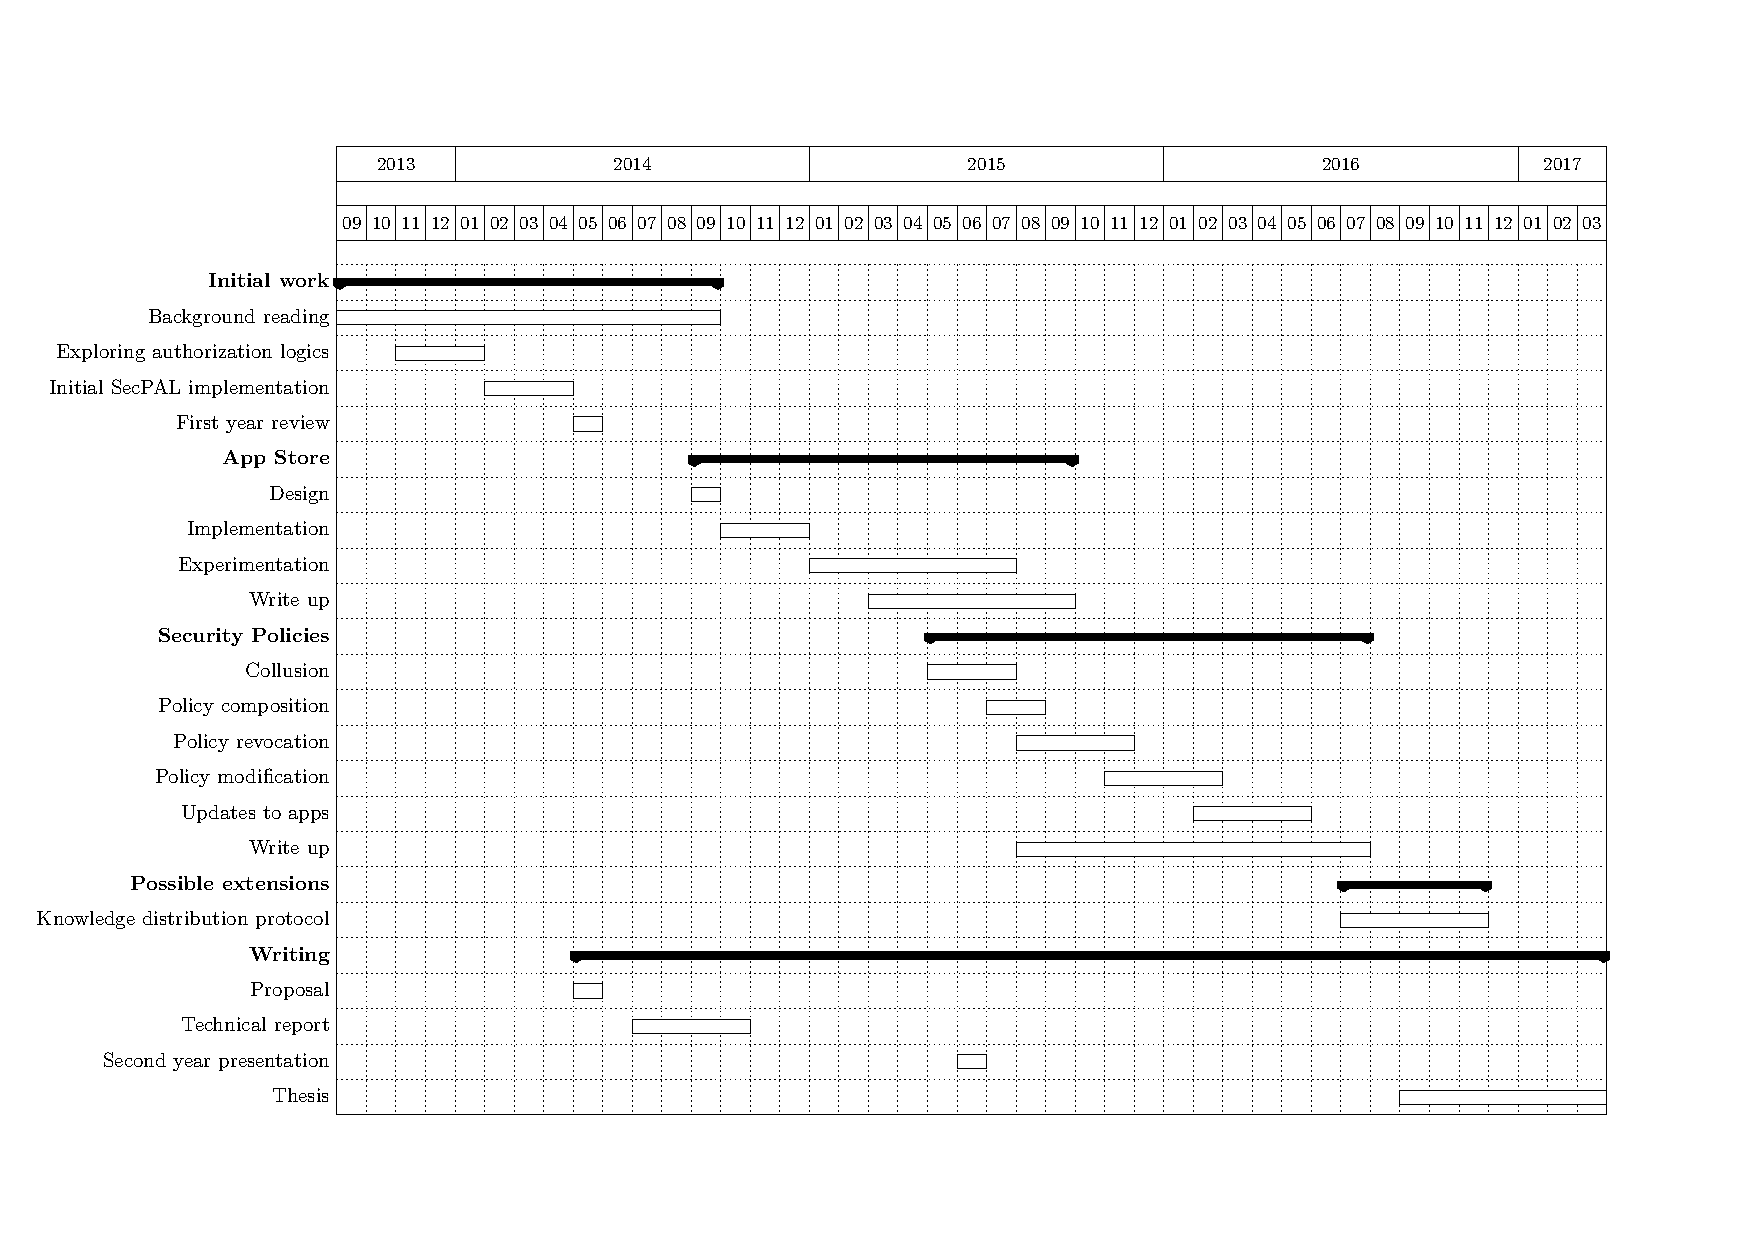
\includegraphics[width=1.4\linewidth,angle=90]{gantt.pdf}
  \caption{Gantt chart showing progress plans throughout funded period of PhD
  study.}
\end{figure*}



\appendix
\bibliography{report}

\end{document}
